\documentclass[]{article}
\usepackage{lmodern}
\usepackage{amssymb,amsmath}
\usepackage{ifxetex,ifluatex}
\usepackage{fixltx2e} % provides \textsubscript
\ifnum 0\ifxetex 1\fi\ifluatex 1\fi=0 % if pdftex
  \usepackage[T1]{fontenc}
  \usepackage[utf8]{inputenc}
\else % if luatex or xelatex
  \ifxetex
    \usepackage{mathspec}
  \else
    \usepackage{fontspec}
  \fi
  \defaultfontfeatures{Ligatures=TeX,Scale=MatchLowercase}
\fi
% use upquote if available, for straight quotes in verbatim environments
\IfFileExists{upquote.sty}{\usepackage{upquote}}{}
% use microtype if available
\IfFileExists{microtype.sty}{%
\usepackage{microtype}
\UseMicrotypeSet[protrusion]{basicmath} % disable protrusion for tt fonts
}{}
\usepackage[margin=1in]{geometry}
\usepackage{hyperref}
\hypersetup{unicode=true,
            pdftitle={Reproducible Research: Peer Assessment 1},
            pdfborder={0 0 0},
            breaklinks=true}
\urlstyle{same}  % don't use monospace font for urls
\usepackage{color}
\usepackage{fancyvrb}
\newcommand{\VerbBar}{|}
\newcommand{\VERB}{\Verb[commandchars=\\\{\}]}
\DefineVerbatimEnvironment{Highlighting}{Verbatim}{commandchars=\\\{\}}
% Add ',fontsize=\small' for more characters per line
\usepackage{framed}
\definecolor{shadecolor}{RGB}{248,248,248}
\newenvironment{Shaded}{\begin{snugshade}}{\end{snugshade}}
\newcommand{\AlertTok}[1]{\textcolor[rgb]{0.94,0.16,0.16}{#1}}
\newcommand{\AnnotationTok}[1]{\textcolor[rgb]{0.56,0.35,0.01}{\textbf{\textit{#1}}}}
\newcommand{\AttributeTok}[1]{\textcolor[rgb]{0.77,0.63,0.00}{#1}}
\newcommand{\BaseNTok}[1]{\textcolor[rgb]{0.00,0.00,0.81}{#1}}
\newcommand{\BuiltInTok}[1]{#1}
\newcommand{\CharTok}[1]{\textcolor[rgb]{0.31,0.60,0.02}{#1}}
\newcommand{\CommentTok}[1]{\textcolor[rgb]{0.56,0.35,0.01}{\textit{#1}}}
\newcommand{\CommentVarTok}[1]{\textcolor[rgb]{0.56,0.35,0.01}{\textbf{\textit{#1}}}}
\newcommand{\ConstantTok}[1]{\textcolor[rgb]{0.00,0.00,0.00}{#1}}
\newcommand{\ControlFlowTok}[1]{\textcolor[rgb]{0.13,0.29,0.53}{\textbf{#1}}}
\newcommand{\DataTypeTok}[1]{\textcolor[rgb]{0.13,0.29,0.53}{#1}}
\newcommand{\DecValTok}[1]{\textcolor[rgb]{0.00,0.00,0.81}{#1}}
\newcommand{\DocumentationTok}[1]{\textcolor[rgb]{0.56,0.35,0.01}{\textbf{\textit{#1}}}}
\newcommand{\ErrorTok}[1]{\textcolor[rgb]{0.64,0.00,0.00}{\textbf{#1}}}
\newcommand{\ExtensionTok}[1]{#1}
\newcommand{\FloatTok}[1]{\textcolor[rgb]{0.00,0.00,0.81}{#1}}
\newcommand{\FunctionTok}[1]{\textcolor[rgb]{0.00,0.00,0.00}{#1}}
\newcommand{\ImportTok}[1]{#1}
\newcommand{\InformationTok}[1]{\textcolor[rgb]{0.56,0.35,0.01}{\textbf{\textit{#1}}}}
\newcommand{\KeywordTok}[1]{\textcolor[rgb]{0.13,0.29,0.53}{\textbf{#1}}}
\newcommand{\NormalTok}[1]{#1}
\newcommand{\OperatorTok}[1]{\textcolor[rgb]{0.81,0.36,0.00}{\textbf{#1}}}
\newcommand{\OtherTok}[1]{\textcolor[rgb]{0.56,0.35,0.01}{#1}}
\newcommand{\PreprocessorTok}[1]{\textcolor[rgb]{0.56,0.35,0.01}{\textit{#1}}}
\newcommand{\RegionMarkerTok}[1]{#1}
\newcommand{\SpecialCharTok}[1]{\textcolor[rgb]{0.00,0.00,0.00}{#1}}
\newcommand{\SpecialStringTok}[1]{\textcolor[rgb]{0.31,0.60,0.02}{#1}}
\newcommand{\StringTok}[1]{\textcolor[rgb]{0.31,0.60,0.02}{#1}}
\newcommand{\VariableTok}[1]{\textcolor[rgb]{0.00,0.00,0.00}{#1}}
\newcommand{\VerbatimStringTok}[1]{\textcolor[rgb]{0.31,0.60,0.02}{#1}}
\newcommand{\WarningTok}[1]{\textcolor[rgb]{0.56,0.35,0.01}{\textbf{\textit{#1}}}}
\usepackage{graphicx,grffile}
\makeatletter
\def\maxwidth{\ifdim\Gin@nat@width>\linewidth\linewidth\else\Gin@nat@width\fi}
\def\maxheight{\ifdim\Gin@nat@height>\textheight\textheight\else\Gin@nat@height\fi}
\makeatother
% Scale images if necessary, so that they will not overflow the page
% margins by default, and it is still possible to overwrite the defaults
% using explicit options in \includegraphics[width, height, ...]{}
\setkeys{Gin}{width=\maxwidth,height=\maxheight,keepaspectratio}
\IfFileExists{parskip.sty}{%
\usepackage{parskip}
}{% else
\setlength{\parindent}{0pt}
\setlength{\parskip}{6pt plus 2pt minus 1pt}
}
\setlength{\emergencystretch}{3em}  % prevent overfull lines
\providecommand{\tightlist}{%
  \setlength{\itemsep}{0pt}\setlength{\parskip}{0pt}}
\setcounter{secnumdepth}{0}
% Redefines (sub)paragraphs to behave more like sections
\ifx\paragraph\undefined\else
\let\oldparagraph\paragraph
\renewcommand{\paragraph}[1]{\oldparagraph{#1}\mbox{}}
\fi
\ifx\subparagraph\undefined\else
\let\oldsubparagraph\subparagraph
\renewcommand{\subparagraph}[1]{\oldsubparagraph{#1}\mbox{}}
\fi

%%% Use protect on footnotes to avoid problems with footnotes in titles
\let\rmarkdownfootnote\footnote%
\def\footnote{\protect\rmarkdownfootnote}

%%% Change title format to be more compact
\usepackage{titling}

% Create subtitle command for use in maketitle
\providecommand{\subtitle}[1]{
  \posttitle{
    \begin{center}\large#1\end{center}
    }
}

\setlength{\droptitle}{-2em}

  \title{Reproducible Research: Peer Assessment 1}
    \pretitle{\vspace{\droptitle}\centering\huge}
  \posttitle{\par}
    \author{}
    \preauthor{}\postauthor{}
    \date{}
    \predate{}\postdate{}
  

\begin{document}
\maketitle

This assignment makes use of data from a personal activity monitoring
device. This device collects data at 5 minute intervals through out the
day. The data consists of two months of data from an anonymous
individual collected during the months of October and November, 2012 and
include the number of steps taken in 5 minute intervals each day.

The data for this assignment can be downloaded from the course web site:

The variables included in this dataset are three:

\begin{enumerate}
\def\labelenumi{\arabic{enumi}.}
\item
  \textbf{steps}: Number of steps taking in a 5-minute interval (missing
  values are coded as \color{red}{\verb|NA|}NA)
\item
  \textbf{date}: The date on which the measurement was taken in
  YYYY-MM-DD format
\item
  \textbf{interval}: Identifier for the 5-minute interval in which
  measurement was taken
\end{enumerate}

The dataset is stored in a comma-separated-value (CSV) file and there
are a total of 17,568 observations in this dataset.

\begin{Shaded}
\begin{Highlighting}[]
\KeywordTok{library}\NormalTok{(readr)}
\KeywordTok{library}\NormalTok{(ggplot2)}
\KeywordTok{library}\NormalTok{(data.table)}
\KeywordTok{library}\NormalTok{(dplyr)}
\end{Highlighting}
\end{Shaded}

\begin{verbatim}
## 
## Attaching package: 'dplyr'
\end{verbatim}

\begin{verbatim}
## The following objects are masked from 'package:data.table':
## 
##     between, first, last
\end{verbatim}

\begin{verbatim}
## The following objects are masked from 'package:stats':
## 
##     filter, lag
\end{verbatim}

\begin{verbatim}
## The following objects are masked from 'package:base':
## 
##     intersect, setdiff, setequal, union
\end{verbatim}

\begin{Shaded}
\begin{Highlighting}[]
\KeywordTok{library}\NormalTok{(patchwork)}
\CommentTok{#library(plyr)}
\end{Highlighting}
\end{Shaded}

Set the working directory to a folder that contains the data

\begin{Shaded}
\begin{Highlighting}[]
\KeywordTok{setwd}\NormalTok{(}\StringTok{"~/Documents/GitHub/RepData_PeerAssessment1"}\NormalTok{)}
\end{Highlighting}
\end{Shaded}

\hypertarget{loading-and-preprocessing-the-data}{%
\subsection{Loading and preprocessing the
data}\label{loading-and-preprocessing-the-data}}

\begin{Shaded}
\begin{Highlighting}[]
\NormalTok{data <-}\StringTok{ }\KeywordTok{fread}\NormalTok{(}\StringTok{"curl https://d396qusza40orc.cloudfront.net/repdata%2Fdata%2Factivity.zip | funzip"}\NormalTok{)}
\end{Highlighting}
\end{Shaded}

\hypertarget{what-is-mean-total-number-of-steps-taken-per-day}{%
\subsection{What is mean total number of steps taken per
day?}\label{what-is-mean-total-number-of-steps-taken-per-day}}

The total number of steps taken per day is \textbf{570,608}

\begin{Shaded}
\begin{Highlighting}[]
\NormalTok{total_number_steps_per_day <-}\StringTok{ }\NormalTok{data[, .(}\DataTypeTok{steps_day=} \KeywordTok{sum}\NormalTok{(steps)), by=}\StringTok{ }\NormalTok{date]}
\KeywordTok{head}\NormalTok{(total_number_steps_per_day)}
\end{Highlighting}
\end{Shaded}

\begin{verbatim}
##          date steps_day
## 1: 2012-10-01        NA
## 2: 2012-10-02       126
## 3: 2012-10-03     11352
## 4: 2012-10-04     12116
## 5: 2012-10-05     13294
## 6: 2012-10-06     15420
\end{verbatim}

Excluding missing data

\begin{Shaded}
\begin{Highlighting}[]
\NormalTok{missing_excluded <-}\KeywordTok{na.omit}\NormalTok{(total_number_steps_per_day}\OperatorTok{$}\NormalTok{steps_day)}
\KeywordTok{sum}\NormalTok{(missing_excluded)}
\end{Highlighting}
\end{Shaded}

\begin{verbatim}
## [1] 570608
\end{verbatim}

\hypertarget{histogram-of-the-total-number-of-steps-taken-each-day}{%
\subsubsection{2. Histogram of the total number of steps taken each
day}\label{histogram-of-the-total-number-of-steps-taken-each-day}}

\begin{Shaded}
\begin{Highlighting}[]
\NormalTok{total_number_steps_per_day_NA <-}\StringTok{ }\NormalTok{data[, .(}\DataTypeTok{steps_day=} \KeywordTok{sum}\NormalTok{(steps)), by=}\StringTok{ }\NormalTok{date]}

\NormalTok{a<-}\KeywordTok{qplot}\NormalTok{(total_number_steps_per_day_NA}\OperatorTok{$}\NormalTok{steps, }\DataTypeTok{geom=}\StringTok{"histogram"}\NormalTok{, }\DataTypeTok{main=}\StringTok{'Number of steps-with NA excluded'}\NormalTok{,}
      \DataTypeTok{fill=}\KeywordTok{I}\NormalTok{(}\StringTok{'pink'}\NormalTok{), }\DataTypeTok{col=}\KeywordTok{I}\NormalTok{(}\StringTok{'pink'}\NormalTok{), }\DataTypeTok{alpha=}\KeywordTok{I}\NormalTok{(}\FloatTok{0.5}\NormalTok{))  }\OperatorTok{+}\StringTok{ }\KeywordTok{xlab}\NormalTok{(}\StringTok{'number of steps'}\NormalTok{) }\OperatorTok{+}\StringTok{ }\KeywordTok{ylab}\NormalTok{(}\StringTok{'density'}\NormalTok{)}
\NormalTok{a}
\end{Highlighting}
\end{Shaded}

\begin{verbatim}
## `stat_bin()` using `bins = 30`. Pick better value with `binwidth`.
\end{verbatim}

\begin{verbatim}
## Warning: Removed 8 rows containing non-finite values (stat_bin).
\end{verbatim}

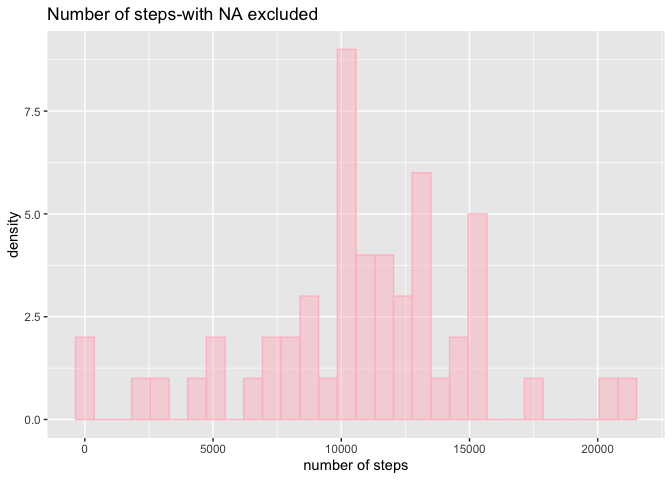
\includegraphics{PA1_template_files/figure-latex/unnamed-chunk-6-1.pdf}

\begin{Shaded}
\begin{Highlighting}[]
\KeywordTok{ggsave}\NormalTok{(a, }\DataTypeTok{file =} \StringTok{'fig.1_histogram_of_total_number_of_steps_day.png'}\NormalTok{)}
\end{Highlighting}
\end{Shaded}

\begin{verbatim}
## Saving 6.5 x 4.5 in image
## `stat_bin()` using `bins = 30`. Pick better value with `binwidth`.
\end{verbatim}

\begin{verbatim}
## Warning: Removed 8 rows containing non-finite values (stat_bin).
\end{verbatim}

\hypertarget{mean-and-median-number-of-each-day}{%
\subsubsection{3. Mean and median number of each
day}\label{mean-and-median-number-of-each-day}}

The mean and median steps taken per day is \textbf{10766.19} and
\textbf{10765} steps respectively.

\hypertarget{mean}{%
\paragraph{Mean}\label{mean}}

\begin{Shaded}
\begin{Highlighting}[]
\KeywordTok{mean}\NormalTok{(missing_excluded)}
\end{Highlighting}
\end{Shaded}

\begin{verbatim}
## [1] 10766.19
\end{verbatim}

\hypertarget{median}{%
\paragraph{Median}\label{median}}

\begin{Shaded}
\begin{Highlighting}[]
\KeywordTok{median}\NormalTok{(missing_excluded)}
\end{Highlighting}
\end{Shaded}

\begin{verbatim}
## [1] 10765
\end{verbatim}

\hypertarget{what-is-the-average-daily-activity-pattern}{%
\subsection{What is the average daily activity
pattern?}\label{what-is-the-average-daily-activity-pattern}}

Here I am calculating mean steps by 5-minute intervals

\begin{Shaded}
\begin{Highlighting}[]
\NormalTok{time_series <-data }\OperatorTok
\StringTok{  }\KeywordTok{replace}\NormalTok{(}\KeywordTok{is.na}\NormalTok{(.), }\DecValTok{0}\NormalTok{) }\OperatorTok\StringTok{  }\CommentTok{# replace NAs with 0 for computation}
\StringTok{  }\KeywordTok{group_by}\NormalTok{(interval) }\OperatorTok
\StringTok{  }\KeywordTok{summarise}\NormalTok{(}\DataTypeTok{steps =} \KeywordTok{mean}\NormalTok{(steps))}
\KeywordTok{head}\NormalTok{(time_series)}
\end{Highlighting}
\end{Shaded}

\begin{verbatim}
## # A tibble: 6 x 2
##   interval  steps
##      <int>  <dbl>
## 1        0 1.49  
## 2        5 0.295 
## 3       10 0.115 
## 4       15 0.131 
## 5       20 0.0656
## 6       25 1.82
\end{verbatim}

\textbf{1. Make a time series plot
(i.e.~\color{red}{\verb|type = "l"|}type = ``l'') of the 5-minute
interval (x-axis) and the average number of steps taken, averaged across
all days (y-axis)}

\begin{Shaded}
\begin{Highlighting}[]
\KeywordTok{ggplot}\NormalTok{(time_series, }\KeywordTok{aes}\NormalTok{(interval, steps)) }\OperatorTok{+}\StringTok{ }\KeywordTok{geom_line}\NormalTok{(}\DataTypeTok{col=}\StringTok{'red'}\NormalTok{) }\OperatorTok{+}\KeywordTok{xlab}\NormalTok{(}\StringTok{'5- Minute intervals'}\NormalTok{) }\OperatorTok{+}\StringTok{ }
\KeywordTok{ylab}\NormalTok{(}\StringTok{'Average steps taken ~ daily'}\NormalTok{) }\OperatorTok{+}\KeywordTok{ggtitle}\NormalTok{(}\StringTok{"Timeseries plot"}\NormalTok{)}
\end{Highlighting}
\end{Shaded}

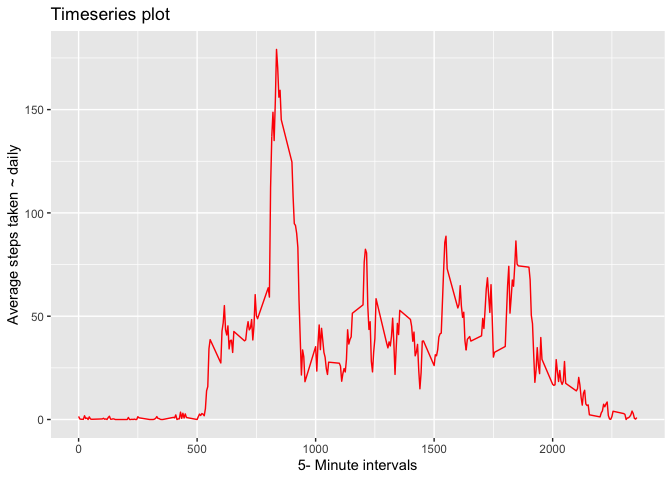
\includegraphics{PA1_template_files/figure-latex/unnamed-chunk-10-1.pdf}

\begin{Shaded}
\begin{Highlighting}[]
\KeywordTok{ggsave}\NormalTok{(}\StringTok{'fig.2_time_series_plot_of_5_munte_interval.png'}\NormalTok{)}
\end{Highlighting}
\end{Shaded}

\begin{verbatim}
## Saving 6.5 x 4.5 in image
\end{verbatim}

\textbf{2. Which 5-minute interval, on average across all the days in
the dataset, contains the maximum number of steps?}

The 5-minute interval that correspons with the maxmum average daily
steps is \textbf{835}

\begin{Shaded}
\begin{Highlighting}[]
\NormalTok{interval_at_max_steps <-}\StringTok{ }\NormalTok{time_series}\OperatorTok{$}\NormalTok{interval[}\KeywordTok{which.max}\NormalTok{(time_series}\OperatorTok{$}\NormalTok{steps)]}
\NormalTok{interval_at_max_steps}
\end{Highlighting}
\end{Shaded}

\begin{verbatim}
## [1] 835
\end{verbatim}

\hypertarget{imputing-missing-values}{%
\subsection{Imputing missing values}\label{imputing-missing-values}}

Note that there are a number of days/intervals where there are missing
values (coded as \color{red}{\verb|NA|}NA). The presence of missing days
may introduce bias into some calculations or summaries of the data.

\textbf{1. Calculate and report the total number of missing values in
the dataset (i.e.~the total number of rows with
\color{red}{\verb|NA|}NAs)}

The steps variable in the dataset has \textbf{2304} missing values

\begin{Shaded}
\begin{Highlighting}[]
\KeywordTok{sum}\NormalTok{(}\KeywordTok{is.na}\NormalTok{(data}\OperatorTok{$}\NormalTok{steps)) }
\end{Highlighting}
\end{Shaded}

\begin{verbatim}
## [1] 2304
\end{verbatim}

\textbf{2.Devise a strategy for filling in all of the missing values in
the dataset. The strategy does not need to be sophisticated. For
example, you could use the mean/median for that day, or the mean for
that 5-minute interval, etc.}

So I'm imputing using a mean for the whole variable. The replica of
orginal data is dat here.

Imputation- the mean over the entire variable is used to impute missing
values

\begin{Shaded}
\begin{Highlighting}[]
\NormalTok{dat <-}\StringTok{ }\NormalTok{data}
\CommentTok{# A <- dat %>% }
\CommentTok{#        group_by(date) %>% }
\CommentTok{#        mutate(steps = ifelse(is.na(steps), }
\CommentTok{#                               mean(steps, na.rm=TRUE), steps))}
\CommentTok{# A}

\CommentTok{# uses mean from all dates where values are recorded}
\NormalTok{dat}\OperatorTok{$}\NormalTok{steps[}\KeywordTok{is.na}\NormalTok{(dat}\OperatorTok{$}\NormalTok{steps)] <-}\StringTok{ }\KeywordTok{mean}\NormalTok{(dat}\OperatorTok{$}\NormalTok{steps, }\DataTypeTok{na.rm=}\OtherTok{TRUE}\NormalTok{)}
\end{Highlighting}
\end{Shaded}

\textbf{3.Create a new dataset that is equal to the original dataset but
with the missing data filled in.}

\begin{Shaded}
\begin{Highlighting}[]
\CommentTok{# uses mean from all dates where values are recorded}
\NormalTok{dat}\OperatorTok{$}\NormalTok{steps[}\KeywordTok{is.na}\NormalTok{(dat}\OperatorTok{$}\NormalTok{steps)] <-}\StringTok{ }\KeywordTok{mean}\NormalTok{(dat}\OperatorTok{$}\NormalTok{steps, }\DataTypeTok{na.rm=}\OtherTok{TRUE}\NormalTok{)}
\NormalTok{dat}
\end{Highlighting}
\end{Shaded}

\begin{verbatim}
##          steps       date interval
##     1: 37.3826 2012-10-01        0
##     2: 37.3826 2012-10-01        5
##     3: 37.3826 2012-10-01       10
##     4: 37.3826 2012-10-01       15
##     5: 37.3826 2012-10-01       20
##    ---                            
## 17564: 37.3826 2012-11-30     2335
## 17565: 37.3826 2012-11-30     2340
## 17566: 37.3826 2012-11-30     2345
## 17567: 37.3826 2012-11-30     2350
## 17568: 37.3826 2012-11-30     2355
\end{verbatim}

\textbf{4. Make a histogram of the total number of steps taken each day
and Calculate and report the mean and median total number of steps taken
per day. Do these values differ from the estimates from the first part
of the assignment? What is the impact of imputing missing data on the
estimates of the total daily number of steps?}

The result is not extremely different, the mean and median are pretty
much closer

\begin{Shaded}
\begin{Highlighting}[]
\NormalTok{total_number_steps_per_day_noNA <-}\StringTok{ }\NormalTok{dat[, .(}\DataTypeTok{steps_day=} \KeywordTok{sum}\NormalTok{(steps)), by=}\StringTok{ }\NormalTok{date]}

\NormalTok{b<-}\KeywordTok{qplot}\NormalTok{(total_number_steps_per_day_noNA}\OperatorTok{$}\NormalTok{steps, }\DataTypeTok{geom=}\StringTok{"histogram"}\NormalTok{, }\DataTypeTok{main=}\StringTok{'Number of steps-no NA'}\NormalTok{,}
      \DataTypeTok{fill=}\KeywordTok{I}\NormalTok{(}\StringTok{'pink'}\NormalTok{), }\DataTypeTok{col=}\KeywordTok{I}\NormalTok{(}\StringTok{'pink'}\NormalTok{), }\DataTypeTok{alpha=}\KeywordTok{I}\NormalTok{(}\FloatTok{0.5}\NormalTok{))  }\OperatorTok{+}\StringTok{ }\KeywordTok{xlab}\NormalTok{(}\StringTok{'number of steps'}\NormalTok{) }\OperatorTok{+}\StringTok{ }\KeywordTok{ylab}\NormalTok{(}\StringTok{'density'}\NormalTok{)}
\NormalTok{a}\OperatorTok{+}\NormalTok{b}
\end{Highlighting}
\end{Shaded}

\begin{verbatim}
## `stat_bin()` using `bins = 30`. Pick better value with `binwidth`.
\end{verbatim}

\begin{verbatim}
## Warning: Removed 8 rows containing non-finite values (stat_bin).
\end{verbatim}

\begin{verbatim}
## `stat_bin()` using `bins = 30`. Pick better value with `binwidth`.
\end{verbatim}

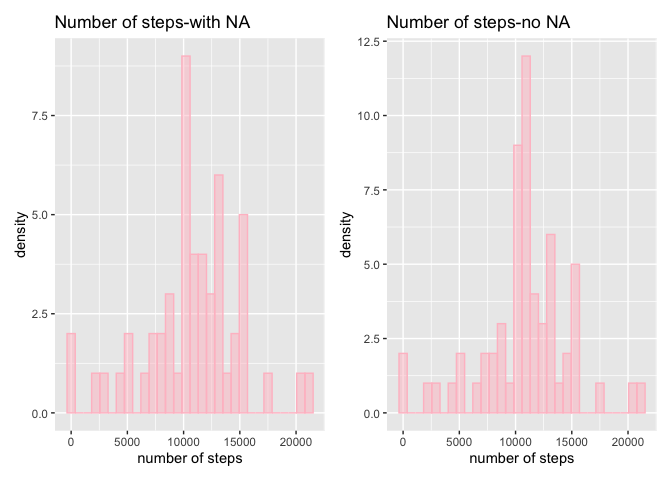
\includegraphics{PA1_template_files/figure-latex/unnamed-chunk-15-1.pdf}

\begin{Shaded}
\begin{Highlighting}[]
\KeywordTok{ggsave}\NormalTok{(b, }\DataTypeTok{file =} \StringTok{'fig.3_histogram_of_total_number_of_steps_day_updated.png'}\NormalTok{)}
\end{Highlighting}
\end{Shaded}

\begin{verbatim}
## Saving 6.5 x 4.5 in image
## `stat_bin()` using `bins = 30`. Pick better value with `binwidth`.
\end{verbatim}

\hypertarget{mean-1}{%
\paragraph{Mean}\label{mean-1}}

\begin{Shaded}
\begin{Highlighting}[]
\NormalTok{total_number_steps_per_day <-}\StringTok{ }\NormalTok{dat[, .(}\DataTypeTok{steps_day=} \KeywordTok{sum}\NormalTok{(steps)), by=}\StringTok{ }\NormalTok{date]}

\KeywordTok{mean}\NormalTok{(total_number_steps_per_day}\OperatorTok{$}\NormalTok{steps)}
\end{Highlighting}
\end{Shaded}

\begin{verbatim}
## [1] 10766.19
\end{verbatim}

\hypertarget{median-1}{%
\paragraph{Median}\label{median-1}}

\begin{Shaded}
\begin{Highlighting}[]
\KeywordTok{median}\NormalTok{(total_number_steps_per_day}\OperatorTok{$}\NormalTok{steps)}
\end{Highlighting}
\end{Shaded}

\begin{verbatim}
## [1] 10766.19
\end{verbatim}

\hypertarget{are-there-differences-in-activity-patterns-between-weekdays-and-weekends}{%
\subsection{Are there differences in activity patterns between weekdays
and
weekends?}\label{are-there-differences-in-activity-patterns-between-weekdays-and-weekends}}

For this part the \color{red}{\verb|weekdays()|}weekdays() function may
be of some help here. Use the dataset with the filled-in missing values
for this part.

\textbf{1. Create a new factor variable in the dataset with two levels
-- ``weekday'' and ``weekend'' indicating whether a given date is a
weekday or weekend day.}

\begin{Shaded}
\begin{Highlighting}[]
\KeywordTok{library}\NormalTok{(lubridate)}
\end{Highlighting}
\end{Shaded}

\begin{verbatim}
## 
## Attaching package: 'lubridate'
\end{verbatim}

\begin{verbatim}
## The following objects are masked from 'package:data.table':
## 
##     hour, isoweek, mday, minute, month, quarter, second, wday,
##     week, yday, year
\end{verbatim}

\begin{verbatim}
## The following object is masked from 'package:base':
## 
##     date
\end{verbatim}

\begin{Shaded}
\begin{Highlighting}[]
\NormalTok{dat}\OperatorTok{$}\NormalTok{date <-}\StringTok{ }\KeywordTok{as.Date}\NormalTok{(dat}\OperatorTok{$}\NormalTok{date)}
\NormalTok{dat}\OperatorTok{$}\NormalTok{dateType <-}\StringTok{ }\KeywordTok{ifelse}\NormalTok{(}\KeywordTok{weekdays}\NormalTok{(dat}\OperatorTok{$}\NormalTok{date) }\OperatorTok\StringTok{ }\KeywordTok{c}\NormalTok{(}\StringTok{"Saturday"}\NormalTok{, }\StringTok{"Sunday"}\NormalTok{), }\StringTok{"weekend"}\NormalTok{, }\StringTok{"weekday"}\NormalTok{)}

\KeywordTok{head}\NormalTok{(dat)}
\end{Highlighting}
\end{Shaded}

\begin{verbatim}
##      steps       date interval dateType
## 1: 37.3826 2012-10-01        0  weekday
## 2: 37.3826 2012-10-01        5  weekday
## 3: 37.3826 2012-10-01       10  weekday
## 4: 37.3826 2012-10-01       15  weekday
## 5: 37.3826 2012-10-01       20  weekday
## 6: 37.3826 2012-10-01       25  weekday
\end{verbatim}

\textbf{2. Make a panel plot containing a time series plot
(i.e.~\color{red}{\verb|type = "l"|}type = ``l'') of the 5-minute
interval (x-axis) and the average number of steps taken, averaged across
all weekday days or weekend days (y-axis). See the README file in the
GitHub repository to see an example of what this plot should look like
using simulated data.}

\begin{Shaded}
\begin{Highlighting}[]
\KeywordTok{ggplot}\NormalTok{(dat, }\KeywordTok{aes}\NormalTok{(}\DataTypeTok{x =}\NormalTok{interval , }\DataTypeTok{y=}\NormalTok{steps, }\DataTypeTok{color=}\NormalTok{dateType)) }\OperatorTok{+}
\StringTok{       }\KeywordTok{geom_line}\NormalTok{() }\OperatorTok{+}\StringTok{ }\KeywordTok{labs}\NormalTok{(}\DataTypeTok{title =} \StringTok{"Panel plots of steps in Weekdays vs Weekends"}\NormalTok{, }\DataTypeTok{x =} \StringTok{"5-minute interval"}\NormalTok{, }\DataTypeTok{y =} \StringTok{"Total Number of Steps"}\NormalTok{) }\OperatorTok{+}\KeywordTok{facet_wrap}\NormalTok{(}\OperatorTok{~}\StringTok{ }\NormalTok{dateType)}
\end{Highlighting}
\end{Shaded}

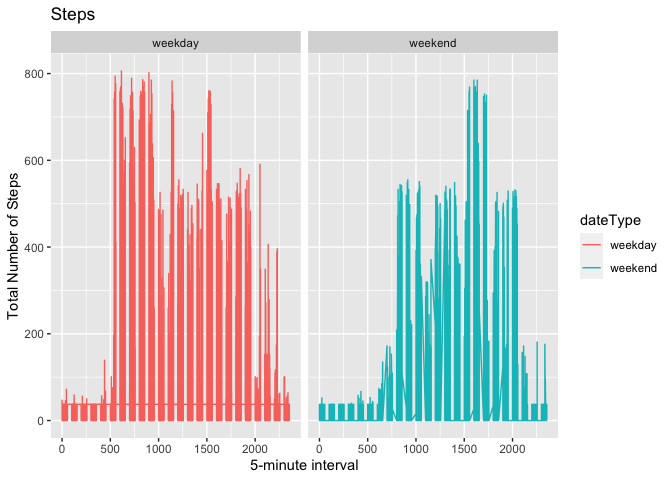
\includegraphics{PA1_template_files/figure-latex/unnamed-chunk-19-1.pdf}

\begin{Shaded}
\begin{Highlighting}[]
\KeywordTok{ggsave}\NormalTok{(}\StringTok{'fig.4_panel_plots.png'}\NormalTok{)}
\end{Highlighting}
\end{Shaded}

\begin{verbatim}
## Saving 6.5 x 4.5 in image
\end{verbatim}


\end{document}
